\documentclass[a4paper]{amsart}
\usepackage{a4wide}
\usepackage[]{graphicx}

\setlength{\parindent}{0.0in}
\setlength{\parskip}{0.1in}

\newcommand{\laplace}[1]{\mathcal{L}\{#1\}}
\newcommand{\Hv}{\textrm{H}}
\renewcommand{\b}{\mathbf}

\begin{document}
\title{6G5Z3011 Multi-variable calculus and analytical methods}
\author{Tutorial Sheet 9}
\maketitle

\textbf{Qs 1 -- 4} on the existence of Fourier series and working with the inner product. \\
\textbf{Qs 5 -- 13} on finding Fourier series and working with odd and even functions.

\begin{enumerate}
  \item
  Consider the inner product $\langle \, , \,  \rangle$ defined by 
  $$ \langle f , g \rangle = \int_{- \pi}^\pi f(x)g(x) \, \, dx .$$
  Show that for every positive integer $n$,
  $$ \langle 1 , p_n \rangle = 0,$$
  where $p_n$ is the function defined by $p_n (x) = \sin (nx)$.
  
  Also, using the formula
  $$\cos A + \cos B = 2 \cos \left (\frac{A+B}{2} \right ) \cos \left (\frac{A-B}{2} \right ) $$
  show that if $m$ and $n$ are positive integers then 
  $$ \langle q_m , q_n \rangle = 
  \left\{
       \begin{array}{lr}
         0, &  \text{ if } m \neq n\\
         \pi, & \text{ if } m = n 
       \end{array}
     \right. ,$$
  where $q_r$ is the function defined by $q_r(x) = \cos (rx)$.
  \item
  For each of the following definitions decide whether the function $f$ will have a Fourier series in the interval $(-\pi, \pi)$. Justify your answers. 
  \begin{enumerate}
  \item
  $$f(x)=\left\{
       \begin{array}{rl}
         -1, &  \text{ if } -\pi < x \leq \frac{-\pi}{2}\\
         0, & \text{ if } \frac{-\pi}{2} < x \leq \frac{\pi}{2} \\
           -1, &  \text{ if } \frac{\pi}{2} < x \leq \pi
       \end{array}
     \right.$$
  \item
  $f(x) = \cos \left ( \frac{1}{x} \right )$
  \item
  $f(x)=8x^4 - 8x^2 + 1$
  \item
  $f(x) = \tan \left ( \frac{1}{x} \right )$
  \end{enumerate}
  \item
  Sketch the graph of the function 
  $$f(x)=\left\{
       \begin{array}{rl}
         1+x, &  \text{ if } -\pi < x \leq 0\\
         2+x, & \text{ if } 0 < x \leq \pi
       \end{array}
     \right. .$$
  What is the value of the Fourier series of this function when (a) $x=1$ and (b) $x=0$?
  \item
  Given that the set of functions
  $$ \{ 1, \sin x, \cos x, \sin 2x , \cos 2x, \sin 3x, \cos 3x , \dots \}$$
  is an orthogonal set with respect to the inner product defined in question (1) above, and that the Fourier series for a function $f$ is given by 
  $$f(x) = \frac{1}{2} a_0 + \sum_{n=1}^\infty a_n \cos nx \, + \, \sum_{n=1}^\infty b_n \sin nx ,$$
  show that 
  $$a_0 = \frac{1}{\pi} \int_{-\pi}^\pi f(x) \, \, dx $$
  and 
  $$ a_m = \frac{1}{\pi} \int_{-\pi}^\pi f(x) \cos mx \, \, dx , \quad (m >0) .$$


  %%%%%%%%%%%%%%%%%%%%%5
  %%%%%%%%%%%%%%%%%%%%%

  \item
Find the Fourier series for the function $f$ which has period $2\pi$ and is defined by 
$$ f(x)=\left\{
     \begin{array}{rl}
       -1, &  \text{ if } -\pi < x \leq 0 \\
       1, & \text{ if } 0 < x \leq \pi 
     \end{array}
   \right.$$
\item
Find the Fourier series for the function $f$, of period $2\pi$, and defined by $f(x)=x$ for $x \in (-\pi,\pi)$.
\item
Find the Fourier series for the function $f$ which has period $2\pi$ and is defined by 
$$ f(x)=\left\{
     \begin{array}{rl}
       0, &  \text{ if } -\pi < x \leq 0 \\
       x, & \text{ if } 0 < x \leq \pi 
     \end{array}
   \right.$$

\item
For each of the following definitions determine whether the function $f$ is odd or even.
\begin{enumerate}
\item
$f(x)=x^3$
\item
$f(x)=e^x$
\item
$f(x)=e^{|x|}$
\item
$f(x)=x \cos x$
\item
$f(x) = (\cos x) (\sin^2 x)$
\end{enumerate}
\item
Prove that the product of two even functions is even and that the product of two odd functions is also even.
\item
Find the Fourier series for the function shown in the diagram below
\begin{center}
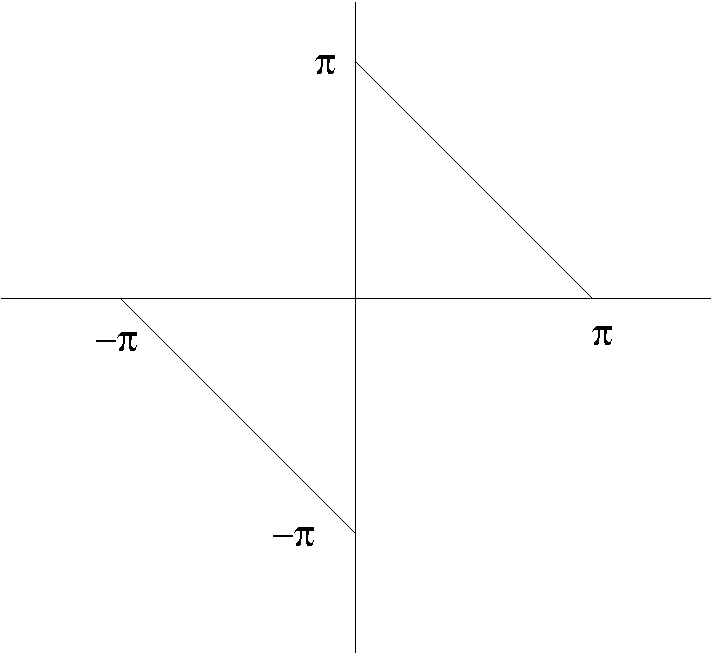
\includegraphics[scale=0.5]{sheet15q6.pdf} 
\end{center}
Verify that the value of the series at $x=0$ is that predicted by Dirichlet's theorem. 
\item
Show that if $h$ is an even and integrable function and $a$ is any positive real number then 
$$ \int_{-a}^a h(x) \, \, dx = 2 \int_0^a h(x) \, \, dx.$$
\item
Find the half range cosine series for the function $f$ defined by $f(x)=x$.
\item
Find the half range sine series for the function $f$ defined by $f(x)=x^2$.
\end{enumerate}


\end{document}